\chapter{Data Storage in Indico}

\par In this chapter, we first look at evolution of storage system in Indico so we mainly turn to ZODB to understand why it was chosen, what it accomplished and where it failed. This chapter, the enlightenment of studying ZODB will be basis for comparison of databases in the next chapter.

\section{The Early Days}

\par Since the early days, Indico has been built around an object-oriented philosophy. In the early 2000's, when the project started, the Object-oriented world and Java in particular seemed to be heading towards a hegemonical position in the software world. Object-oriented philosophy managed to permeate into practically all fields of computer science, including, of course, web applications, which until then had been no more than collections of CGI scripts in several interpreted languages (which is the number one reason of why PHP is still so popular, isn't it?).

\par Choosing Python as the development language for a new web application could have seemed a risky option in 2002, when buzzwords like "Django" or "Flask" were everything but real, but risk has shown to pay off in the long term: the Python web ecosystem is now flourishing and Indico is part of this movement. This means that months of development time can now be saved in the implementation of certain complex features since a full ecosystem of libraries and applications that were not there one decade ago emerged.

\par From the beginning, one of the most important (if not the most important) dependencies of Indico has been ZODB. While practically all the main dependencies have been replaced over time, from XML libraries to web frameworks, not to mention JavaScript libraries and templating engines, ZODB has stayed in. It's not hard to imagine that this was due to the fact that ZODB occupies a primordial role in the software package, by providing a transparent persistence layer over which the business logic of Indico is implemented.

\par Once again, the choice of ZODB as data storage solution for Indico was daring, to say the least. Despite the growing popularity of the project in the early 2000's (mainly due to the increasing usage of the Zope framework), non-relational DBs were far from being considered mainstream. The enthusiasm around object-oriented data stores seemed to be increasing, but the following decade would show a clear predominance of relational databases over the competition.

\section{The Decade of ZODB} 

\par In 10 years of ZODB usage, a single serious incident due to a database problem was reported. It caused a service interruption of around one day, the only one to report in a decade. Many other minor incidents have happened, but never related to the DB itself or the technology behind it. In addition to that, there are no examples of data corruption to talk about. This said, it is not unfair to say that ZODB is a reliable product, a solid storage solution that can be trusted upon.

ZODB is a glorified pickle store. This is both its strength and its weakness: it is intrinsically bound to Python and its Object-oriented subsystem. This provides a great degree of transparency and the expressiveness of an Object-oriented approach, but sacrifices, first of all, portability and, additionally (but also of great importance), the performance of some operations.

As an example, let's take a very simple DB operation that is usually taken for granted in the relational world: getting the list of names of all registrants in a conference:

\begin{lstlisting}[language=SQL]
  SELECT last_name, first_name
  FROM conference_attendants
  WHERE conf_id = 1234;
\end{lstlisting}

This type of query can be performed in ZODB, but it will involve:

\begin{itemize}
  \item Querying the DB for all the objects relative to attendants of the conference in question. This involves:

  \begin{itemize}
    \item Retrieving the Conference object from the DB
    \item Reconstructing the object from its serialized form (pickle)
    \item Extracting the list of objects from the Conference object and requesting each one of them from the DB
  \end{itemize}
  \item Reconstructing (unpickling) the objects client-side
  \item Retrieving the attributes in question from the reconstructed object.
\end{itemize}

These are by no means slow operations. Specifically, Point 1 involves a significant amount of network latency (given that each object is requested separately) and Point 2 can be significantly slow if a large amount of objects is involved.

This is the main issue with ZODB: objects are separate entities and, even though there are tricks that allow us to group/retrieve them together, those are not without their own disadvantages.

Of course there are advantages to the Object-oriented approach: it's easy to work with and there is no need for conversion mechanism that will map classes in the object domain to database tables and rows. This mechanism is normally called "ORM" (Object-Relational Mapping) and is nowadays a common feature of many web frameworks (Ruby on Rails, Django, Symfony, etc.).

\subsection{The Age of Caching}

Over the last 5 years, Indico has gradually become ubiquitous at CERN. The addition of a room booking module and later video-conferencing capabilities has for sure contributed to the broadening of the tool's audience. This has quickly increased the load over the system, and consequently the database. After a round of DB optimization fixes and several studies into ZODB, developers quickly realized that future growth needed to be sustained by a different strategy.

Performance improvement could be easily achieved in two different ways:

\begin{itemize}
  \item Faster DB access - this would depend on both the speed of the network connection between the DB and the web workers and the performance of the DB server instead. The choice was made of equipping the Indico DB server with SSD devices.
  \item Less frequent DB access - this would rely on keeping more data on the client side and asking for DB content less often, also known as "caching", and ZODB already has a client cache. Unfortunately, it is per-process cache and state is not shared between caches. An application-level caching layer was implemented, which can use different caching backends.
  \item DB replication - this could provide some relief to the main DB server during activity peaks, specifically by adding a second ZODB server that would mirror it. Web workers wanting to retrieve data could then contact to the second server instead of the first one, thus freeing the latter from keeping additional connections open for them.
\end{itemize}

Unfortunately, no simple and stable ZODB/ZEO replication mechanism was available at the time. The only exception was ZRS, which was a commercial product. An evaluation version was requested and it proved to be an effective solution. Its high price was the only deterring factor. It was decided that, for the moment, the first two solutions would be implemented. ZRS has recently been open sourced by Zope, which makes it a quite viable option for the future.

After a first implementation of caching with recourse to files, memcached support was finally added, which allowed for further performance improvements. Later, Redis support would be added.

At the time of the writing of this article, caching is being used in several parts of the application, including conference timetables and the room booking system. Furthermore, new (more experimental) features such as the Dashboard are making use of specific forms of caching (Redis, in this case) in order to keep a secondary, fast, easy to query secondary storage. However, it also comes with its own problems; data must be synchronized with main DB which requires extra overhead for writes and maintenance cost of extra code (7 Lua scripts for server-side queries).
 
\section{The Need for a New Storage}

The evolution of Indico's feature set has been increasingly towards a more personal, user-centered application with an emphasis on the events that matter to each particular user. The User Dashboard is a perfect example of the kind of feature that users can expect in the future from the system: a page that allows them to see which events are going on that involve them, as well as those taking place in their favorite categories.

Needless to say that the implementation of this kind of functionality implies the existence of mechanisms that allow a significant volume of information to be quickly queried and all matches retrieved. It is necessary to find out which events match a specific condition in a universe of hundreds of thousands (or potentially more) of them. This brings us to the problem of indexing.

\subsection{Indexing}

One of the most important features of a relational database is that arbitrary queries can be executed at any time. This allows for a great degree of flexibility, but makes things less predictable on the server side - a server has to know what to expect, otherwise it will take too much time going through all elements and checking whether they fit the criteria. Fortunately, most RDBMSs support database indexes and allow them to be created at the stroke of a key. Indexes allow results to be retrieved much more quickly at the cost of a small performance penalty on write operations.

ZODB provides developers with several database-targeted data structures. Examples of that are \textit{BTree } and \textit{TreeSet} (implemented using BTrees), two structures aimed at large volumes of data that need to be stored in chunks and accessed in sub-linear time. BTrees are implemented on top of the Object-Oriented storage paradigm of ZODB (in separate "buckets", the nodes of the B-Tree). One important detail is that the ZODB server application implements no additional logic regarding these data structures - it handles objects in a pretty transparent way, simply retrieving them as they are requested. This is not completely true, as conflict resolution is done by the database itself and can be overridden by custom library code. All searches, comparisons and even changes on DB objects are, however, performed on the client side, and only then reflected in the database.

The simplified logic on the server side together with the absence of a feature that can be compared to "stored procedures" leave the developer no other option than implementing everything on the client side. While this can be seen as a way of keeping things simple, it is highly inefficient as it implies the presence of all the relevant objects in the local context. This can be extremely slow for large data structures.

As a result, while implementing indexes in ZODB is possible, these are also potentially much slower than their relational counterparts, not to mention that they have to be implemented at the application level, even though ZODB can persist them for future use. There are tools that help developers with this task, such as \textit{zope.index} and \textit{repoze.catalog}, but they do not solve the problem of having to implement the full query logic on the client side.

\subsection{An Example: The Dashboard}
 
The User Dashboard has been the first Indico module to be implemented on a storage mechanism that is not ZODB-based (Redis). While ZODB remains as the primary source of information for user-event relations, Indico is fetching this data directly from a Redis server, and updating it in parallel with Indico. Redis acts here as a "write-through" cache, a secondary data store that is, however, always up-to-date.

There are reasons for this choice. They are mostly connected to the relation between the different entities in the problem.

\hfill 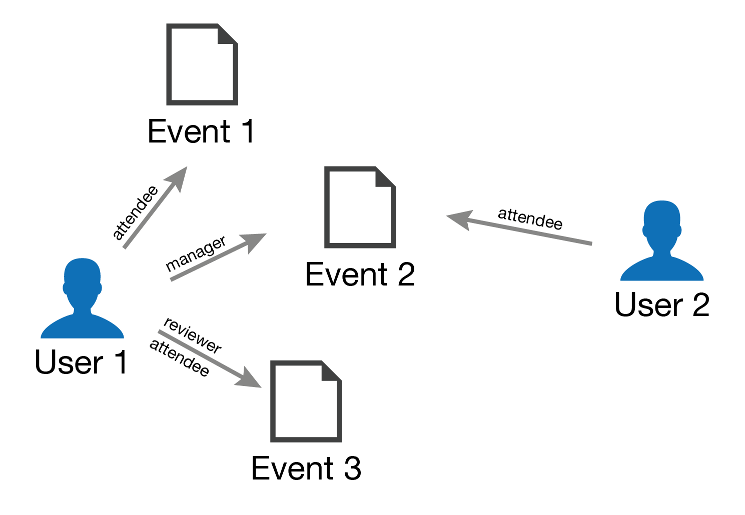
\includegraphics[scale=1]{2/figures/dashboard.png}

The Dashboard is basically a time-ordered display of the relationships between a particular user and certain events. For instance, User 1 is an attendee of Event 1 or the manager of Event 2. Logically, other users can share the same role in the context of the same event - it's a many to many relationship. ZODB has no problem in defining many-to-many relationships - its OO-oriented approach allows references to be added pretty much anywhere, very much like in a graph - that is not the issue. However, there are actually two problems:

\begin{enumerate}
  \item It has already been mentioned before that ZODB fetches objects separately, so it is impossible to retrieve 100 pickled persistent Conference objects in one go.
  \item Indexing, once again, is hard and not optimal
\end{enumerate}

A possible (naive) approach for a ZODB-based solution to this problem would be creating a BTree, ordered by time and event ID, containing the conference objects that relate to a particular user. If we wanted to concentrate everything in a single BTree, we could just use a composite key such as (\textit{user\_id, timestamp, event\_id, role}). This would allow us to effectively query events by user/timestamp. Still, it would be necessary to ask for and unpickle every single object for which a reference is returned (problem 1). Now, let's assume that problem 1 has minimal impact in terms of performance (which is not exactly true, but let's assume it just for the sake of the argument):

\begin{itemize}
  \item Querying by user would be OK - It's a simple range query on $(user_id, 0, '', '')$
  \item Querying by timestamp for a particular user would be OK: range query on $(user_id, timestamp, '', '')$
  \item Creating a new entry would be trivial - it would just be a matter of adding a new key to the tree, and the worst case scenario would be a bucket split/join operation, which would be far from disastrous performance-wise
  \item Deleting a user would be OK - it would be a matter of finding out all corresponding keys using a range query and deleting them (O(N))
  \item Detaching a user from a role would be possible in O(N)
  \item Completely detaching a user from a particular event would be simple, as it is a subproblem of the previous problem
\end{itemize}

There are, however, some operations that are not as simple:

\begin{itemize}
  \item If \textbf{an event gets deleted}, one will need to remove all index entries that refer to it $-$ using this approach, that means going over all $user_ids$ and checking whether the event is present
  \item Same happens if an event changes start date - the timestamp will change and one will need to update all corresponding entries
\end{itemize}

These are potential blockers, since event deletion is not such an uncommon operation. Of course there are known solutions to this problem, such as:

\begin{itemize}
  \item Marking the event as deleted and excluding deleted events from query results. The deletion of "old" events from the index could then be made in the background by a periodic job that would go over all users. This wouldn't solve the start date issue, though.
  \item Having a reverse-lookup index that would map event ids to the corresponding keys in the primary index. This means that we would know that Event 2 has index keys (User 1, 12365, Event 2, manager) and (User 2, 12345, Event 2, attendee). This helps with both situations, but it's far from ideal as one would have to maintain two indices instead of one.
\end{itemize}

Similar problems have already been solved in the past using the second approach. In fact, a helper module (Catalog) was written, based on ZODB BTrees, that makes it easier for developers to deal with indexes, by abstracting some of the needed operations (like, for instance, maintaining a reverse-lookup index). However, debugging such index code is not an easy task.

\begin{table}[t]
	\centering
    \begin{tabular}{ | c | l |}
    \hline
    \textbf{Limitation} & \textbf{Explanation} \\ \hline
    Ad-hoc queries & ... \\ \hline
    Indexing & ... \\ \hline
    Caching on the Server Side & ... \\ \hline
    Replication & ... \\ \hline
    Community & ... \\ \hline
    \end{tabular}
    \caption{Limitations of ZODB}
    \label{limitations}
\end{table}

To sum up, saved data is hierarchical and contains highly interrelated connections between entities so that they can be accessed from many different points. Therefore, ability of querying arbitrarily and doing projections is vital from performance point of view. Overcoming this problem is possible via caching but it risks consistency of data and brings maintenance burden of extra code which means developers are working in spite of DB, not for new features with the support of DB. Rapid development, the reason of why ZODB is chosen at first isn't true any more. Moreover, its community is small, documentation and development speed is lacking. Last but not least, it is still a niche product even after 10 or so years.

It seems to be clear, from what was mentioned above, that ZODB is not an optimal solution for this class of data problem.

\section{Selection Criterias of New Database}

There are mainly 6 categories:

\begin{enumerate}
  \item \textit{Availability}: Replacement technology must be open source since Indico is an open source application, users can not be forced to use a commercial solution. Moreover, DB license should comply with the licenses of other software packages used.
  \item \textit{Scalability / Replication}: Scalability is the main driving factor for the replacement of ZODB so it is a must in the system due to increasing usage and popularity of Indico. DB should have room for extensibility for the foreseeable future.
  \item \textit{Ease of Use / Development}: DB should have good tool support for Python, main development language of Indico and it should decrease the time to implement new features so it should be transparent as much as possible like ZODB. Complexity of a feature should be come from application logic, not the commanding DB for data.
  \item \textit{Transactions / Consistency}: Writes touch many entities at the same time due to devilish dependencies between entities. Thus, transaction capability of DB is deadly important to keep data consistent.
  \item \textit{Community / Momentum}: Indico aims solving conference management problem, not the nitty gritty use-case details of a specific DB. When a problem is encountered, respective solution should mostly have been studied before. Successful deployments are an important representative of this requirement.
  \item \textit{Cost / Exit Strategy}: Transition costs should be minimized and also dependency to DB should be as low as possible to decrease the exit cost when time to pay technical debt has come.
\end{enumerate}

It is easily seen that ZODB isn't doing good because it is successful at only 2 criterias of 6; namely, being open source and transaction support.

% ---------------------------------------------------------------------------
% ----------------------- end of thesis sub-document ------------------------
% ---------------------------------------------------------------------------